\documentclass[]{article}
\usepackage{lmodern}
\usepackage{amssymb,amsmath}
\usepackage{ifxetex,ifluatex}
\usepackage{fixltx2e} % provides \textsubscript
\ifnum 0\ifxetex 1\fi\ifluatex 1\fi=0 % if pdftex
  \usepackage[T1]{fontenc}
  \usepackage[utf8]{inputenc}
\else % if luatex or xelatex
  \ifxetex
    \usepackage{mathspec}
  \else
    \usepackage{fontspec}
  \fi
  \defaultfontfeatures{Ligatures=TeX,Scale=MatchLowercase}
\fi
% use upquote if available, for straight quotes in verbatim environments
\IfFileExists{upquote.sty}{\usepackage{upquote}}{}
% use microtype if available
\IfFileExists{microtype.sty}{%
\usepackage[]{microtype}
\UseMicrotypeSet[protrusion]{basicmath} % disable protrusion for tt fonts
}{}
\PassOptionsToPackage{hyphens}{url} % url is loaded by hyperref
\usepackage[unicode=true]{hyperref}
\hypersetup{
            pdfborder={0 0 0},
            breaklinks=true}
\urlstyle{same}  % don't use monospace font for urls
\usepackage{graphicx,grffile}
\makeatletter
\def\maxwidth{\ifdim\Gin@nat@width>\linewidth\linewidth\else\Gin@nat@width\fi}
\def\maxheight{\ifdim\Gin@nat@height>\textheight\textheight\else\Gin@nat@height\fi}
\makeatother
% Scale images if necessary, so that they will not overflow the page
% margins by default, and it is still possible to overwrite the defaults
% using explicit options in \includegraphics[width, height, ...]{}
\setkeys{Gin}{width=\maxwidth,height=\maxheight,keepaspectratio}
\IfFileExists{parskip.sty}{%
\usepackage{parskip}
}{% else
\setlength{\parindent}{0pt}
\setlength{\parskip}{6pt plus 2pt minus 1pt}
}
\setlength{\emergencystretch}{3em}  % prevent overfull lines
\providecommand{\tightlist}{%
  \setlength{\itemsep}{0pt}\setlength{\parskip}{0pt}}
\setcounter{secnumdepth}{0}
% Redefines (sub)paragraphs to behave more like sections
\ifx\paragraph\undefined\else
\let\oldparagraph\paragraph
\renewcommand{\paragraph}[1]{\oldparagraph{#1}\mbox{}}
\fi
\ifx\subparagraph\undefined\else
\let\oldsubparagraph\subparagraph
\renewcommand{\subparagraph}[1]{\oldsubparagraph{#1}\mbox{}}
\fi

% set default figure placement to htbp
\makeatletter
\def\fps@figure{htbp}
\makeatother


\date{}

\begin{document}

\section{Chap.1 Introduction}\label{header-n0}

 改善图示信息以便人们解释;
为存储、传输和表达而对图像数据进行处理,以便于机器自动理解。
数字图像处理是借助于数字计算机处理数字图像
\(\qquad\)\(\qquad\)图像源:从伽马射线到无线电波的整个电磁波谱,包括超声波`电子显微镜和计算机生成的图像
电磁能谱,声波、超声波、电子 图像处理-图像分析/理解-计算机视觉 的连续统
低级-中级-高级 处理

\subsubsection{1.2 起源}\label{header-n10}

 电缆传输图片 计算机的兴起 空间项目的开发 CT(计算机断层)

\subsubsection{1.3 实例应用}\label{header-n16}

\subsubsection{1.4 基本步骤}\label{header-n17}

 输入-输出都是图像 输入图像-输出提取的属性

\(\qquad\)\(\qquad\)\emph{Figure 1.23} 图像获取image acquisition
图像增强(image enhancement):使图像在特定应用中比原始图像更适合进行处理
图像复原(image restoration):倾向于以图像退化的数学或概率模型为基础
彩色图像处理(color image processing)
小波:以不同辨率来描述图像的基础(wavelets and multiresolution
processing) 压缩(compression) 形态学处理(morphological processing)
分割(segmentation) 表示(representation
确定表示范围,比如边界或者整个区域)与描述(description 特征选择)
识别(recognition):基于目标的描述给该目标赋予标志 显示(display)

\subsubsection{1.5 图像处理系统的组成}\label{header-n34}

 \emph{Fig. 1.24}

\section{第2章 数字图像基础}\label{header-n37}

\subsubsection{2.1 人类视觉系统}\label{header-n40}

 人眼结构\\
 眼中图像的形成\\
 亮度适应和辨别\\

\subsubsection{2.2 光和电磁波谱}\label{header-n46}

 E=hv 光子 频率段\\
 单色光/无色光 的唯一属性是 强度,用 灰度级 表示,从黑到白的度量
值通常称为 灰度级\\
 彩色光源:发光强度(能量总和,瓦特)
光通量(流明数,观察者从光源感受到的能量) 亮度(主观描述)\\
 要求``看到''一个物体的电磁波的波长必须小于等于物体的尺寸\\

\subsubsection{2.3 图像感知和获取}\label{header-n53}

 照射源, 场景\\
 照射可以由非传统光源,比如超声波甚至计算机产生的照射模式。\\
 平坦表面反射 透射\\
 \(\qquad\)\(\qquad\)\(\qquad\)单个传感器,条带传感器,阵列传感器\\
 简单的图像形成模型 2.3.4\\
 反射系数/透射系数 * 入射分量\\
 灰度级/强度级 \(l=0\)黑色 \(l=L-1\)白色 gray scale\\

\subsubsection{2.4 取样和量化}\label{header-n63}

 取样:对坐标值进行数字化 =》样本数\\
 量化:对幅值数字化 =》灰度级\\
 实践中,取样方法由生成该图像的传感器配置决定\\
 \(\qquad\)\(\qquad\)\(\qquad\)二维阵列 \(f(x,y)\)
三种表示\emph{Fig2.18}\\

 图像原点位于左上角:图像显示器, 矩阵排列方式\\

 \(M:row\; N:col\) \(L\):灰度级,一般为2的整数次幂\\
 \emph{动态范围}: 最大可度量灰度与最小可检测灰度之比 dynamic range\\
 \emph{饱和度}:超过该值的灰度级会被剪切掉 saturation\\
 \emph{对比度}:最高和最低灰度级的灰度差;高动态范围意味着高对比度
contrast\\

\(\qquad\)\(\qquad\)\(\qquad\)\emph{空间分辨率}的度量必须针对空间单位来规定才有意义
spatial resolution \emph{灰度分辨率}:
灰度级中可分辨的最小变化,最通用8比特 intensity resolution
\(\qquad\)\(\qquad\)\(\qquad\)\emph{内插}:
使用已知数据来估计未知位置的数值的处理 interpolation
最近邻内插,把元图像中最近邻的灰度赋给每个新位置 nearest neighbor
interpolation 双线性内插 bi-linear interpolation 双三次内插 bicubic
interpolation

\subsubsection{2.5 像素间的关系}\label{header-n86}

 4邻域 8邻域 4/8-neighbors
\(\qquad\)\(\qquad\)\(\qquad\)\textbf{邻接性}:
处于同一灰度值集合且处于邻域中 adjacency 4/8/m-adjacency
\textbf{连通性}: 相互邻接的 Connectivity 用连通定义 \emph{前景} 和
\emph{背景} foreground background
\textbf{区域边界}:与背景有邻点的像素集合(8邻接)(boundary, border,
contour) \emph{内边界}与\emph{外边界}(背景边界)(inner/outer border)
the concept of edge is different from boundary, and is formed from
pixels with derivative values that exceed a preset threshold
\(\qquad\)\(\qquad\)\(\qquad\)距离度量的定义,欧式距离、D4距离、D8距离

\subsubsection{2.6 数学工具}\label{header-n99}

 灰度的集合运算P47 \textbf{并集}:对应最大 交集:对应最小 补集:差值
\(\qquad\)\(\qquad\)\(\qquad\)\textbf{模糊集}: 引入\emph{隶属度函数}
Fuzzy set, membership function \textbf{几何变换}P109 Geometric spatial
transformation \textbf{反向映射与前向映射} forward/inverse mapping
\textbf{图像对齐\图像配准},选择约束点 image registration, tie
points/control points 将图像作为向量处理 \textbf{图像变换}P54-56 image
transform

\section{Chap.3 Intensity Transformations and Spatial
Filtering}\label{header-n110}

\(\qquad\)\textbf{spatial domain}: the image plane itself\\
 \(\qquad\)\textbf{transform domain}: transforming an image into the
transform domain doing the processing there and bring the results back
into the spatial domain, e.g. \emph{frequency domain}

\(\qquad\)Two principal categories of \emph{spatial processing}:

\begin{enumerate}
\def\labelenumi{\arabic{enumi}.}
\item
  \textbf{intensity transformation}: operate on single pixels
\item
  \textbf{spatial filtering}: performs operations by working in a
  neighborhood of every pixel in an image
\end{enumerate}

\subsection{3.1 Background}\label{header-n123}

\[g=T[f]\]

where \(f\) is the input image, \(g\) is the output and \(T\) is an
operatior on \(f\)

e.g. averaging out the intensities of all pixels in a neighborhood,
called \emph{spatial filtering}, with which operation called
\emph{spatial filter} , a.k.a. \emph{spatial mask}, \emph{kernel},
\emph{template}, \emph{window}. It's a \emph{neighborhood processing}

\(\qquad\)Let the window shrink to one pixel and this becomes
\emph{point processing}.

\(\qquad\)\textbf{Enhancement}: the process of manipulating an image so
that the result is more suitable than the original for a specific
application, implying it's problem-oriented. No general theory.

\subsection{3.2 Some Basic Intenisty Transformation
Fucntions}\label{header-n133}

\[s=T(r)\]

Three basic types:

\begin{enumerate}
\def\labelenumi{\arabic{enumi}.}
\item
  Linear (negative and identity)
\item
  Logarithmic (log and inverse-log)
\item
  Power-law (nth power and nth root)
\end{enumerate}

Image Negatives

\[s=L-1-r\]

Particularly suited for enhancing white or gray detail embedded in dark
regions, especially when the black areas are dominant in size.

Log Transformations

\[s=c\;log(1+r)\]

where \(c\) is a constant and \(r\geq0\). It maps a narrow range of low
intensity values in the input into a wider range of output levels, and
the opposite is true of higher values of input levels. Use this to
expand the values of dark pixels in an image while compressing the
higher level values. The opposite is true of the inverse log. E.g.
processing Fourier spectra.

Power-Law(Gamma) Transformation

\[s=cr^{\gamma}\]

where \(c\) and \(\gamma\) are postive constants

Sometimes also written as

\[s=c(r+\epsilon)^{\gamma}\]

Varying \(\gamma\) gives different transformation.

Applications: \textbf{Gamma correction}: the process to correct
power-law response phenomena. e.g. CRT gamma correction
\textbf{General-purpose contrast manipulation}

Piecewise-Linear Transformation Functions

\(\qquad\)A complementary approach to the methods above, and it can be
arbitrarily complex.

\textbf{Contrast stretching}; expands the range of intensity levels in
an image so that it spans the full intensity range of the recording
medium or display device.

\(\qquad\)if \(r_1=s_1\quad\quad s_2=r_2\), it becomes a thresholding
function

\textbf{Intensity-level slicing}: highlighting a specific range of
intenisties in an image. This produces a binary image and is useful for
studying the shape of the flow of the contrast medium.

\textbf{Bit-plane slicing}: highlighting certain bits of the intensities
of a byte. The higer order bit planes contain a significant amount of
the visually significant data, the lower-order planes contribute to more
subtle intensity details. Decomposing an image into its bit planes is
useful for analyzing the relative importance of each bit in the image, a
process that aids in determining the adequacy of the number of bits used
to quantize the image. Also useful for iamge compression, in which fewer
tan all planes are used in reconstructing an image.

\subsection{3.3 Histogram Processing}\label{header-n178}

\(\qquad\)\textbf{Histogram}: a digital image with intensity levels in
the range \([0,L-1]\) is a discrete function \(h(r_k)=n_k\), where
\(r_k\) is the kth intensity value and \(n_k\) is the number of pixels
in the image with intensity \(r_k\). Commonly normailzed by the total
number of pixels \(MN\), i.e. \(p(r_k)=n_k/MN\) ,which is an estimate of
the probability of occurrence of intensity level in an image.

\(\qquad\) Basis for numerous spatial domain processing techniques.
\(\qquad\) For image enhancement \(\qquad\) the information inherent in
histograms is useful in other image processing applicaitons, e.g. image
compression.

Dark, light, low contrast and high contrast on their histograms

Histogram Equalization

\textbf{PDF}, \textbf{CDF}

\[s=T(r)\quad0\leq r\leq L-1\]

Assume that:

\begin{enumerate}
\def\labelenumi{\arabic{enumi}.}
\item
  \(T(r)\) is a monotonically increasing function sometimes strictly
  monotinically increasing 
\item
  \(T(r)\) is surjective
\end{enumerate}

Since CDF satisfies condtion 1 and 2, we have

\[s=T(r)=(L-1)\int\limits^{r}_0 p_r(w)dw\]

which, by simple calculus, is proved to give rise to the result below:

\[p_s(s)=\dfrac{1}{L-1}\quad0\leq s\leq L-1\]

That is, given any \(p_r(r)\), \(p_s(s)\) always is uniform, independent
of \(r\).

\(\qquad\)For the discrete counterpart

\[p_r(r_k)=\dfrac{n_k}{MN}\quad k=0,1,2,...,L-1\\
s=T(r_k)=(L-1)\sum\limits^k_{j=0}p_r(r_j)\\
\qquad\qquad\quad\quad=\dfrac{L-1}{MN}\sum\limits^k_{j=0}n_j\quad k=0,1,2,...,L-1\\
s \; needs\ to\ be\ rounded\ to\ the\ nearest\ integer\]

\(\qquad\)\(Eq. (10)\) is called \textbf{histogram equalization} or
\textbf{histogram linearization}. Though it cannot be proved in general
that discrete histogram equalization. It has the general tendency to
spread the histogram of the input image so that the intensity levels of
the equalized image space wider range of the intensity scale. The net
result is \emph{contrast enhancement}.

Histogram Matching/specification

\(\quad\quad\) It is useful sometimes to be ablle to specify the shape
of the histogram that we wish the processed image to have, not always a
uniform one.

\(\quad\quad\) Either in continuous cases or in discrete cases,
histogram mathcing is achieved through an imtermediate stage of
histogram equalization. That is, given the input \((r, p_r)\) and the
specified output \((z,p_r)\), we obtain the mapping from \(r\) to \(z\)
by equalize their corresponding histogram equalized results.

\begin{quote}
\begin{enumerate}
\def\labelenumi{\arabic{enumi}.}
\item
  Conpute the corresponding histogram-equalized results of \(r\) and
  \(z\) , denoted by \(s_k\) and \(G(z_q)\), discretize them
\item
  For \(k=1,...L-1\)

   Find the closest \(G(z_q)\) to \(s_k\) Map this \(k\) to this \(q\)
  if there are more than one \(q\) choose the smallest one
\item
  The mapping from \(r_k\) to \(z_q\) is thus obtained
\end{enumerate}
\end{quote}

\(\quad\quad\) Histogram specification is, for the most part, a trial
and error process, and there are no rules for specifying histograms and
one must resort to analysis on a case-by-case basis for any given
enhancement task.

Local Histogram Processing

\(\quad\quad\) It is necessary to enhance details over small
\emph{areas} in an iamge. The solution is to devise transformation
functions based on the intensity distribution in a neighborhood of every
pixel in the image

\(\quad\quad\) The histogram is computed over a neighborhood while the
transformation is done only at the center.

Using Histogram Statistics for Image Enhancement

\emph{mean}, \emph{moment}, \emph{variance} obtained from the histogram
\emph{sample mean}, \emph{sample variance} obtained directly from the
image

Mean: intensity Variance; contrast global and local

\(\quad\quad\) Using the local mean and variance can develop simple yet
powerful enhancement techniques based on statistical measures that have
a close, predictable correspondence with image appearance.

\(\quad\quad\) A contrast enhancing application

\subsection{3.4 Fundamentals of Spatial Filtering}\label{header-n254}

\(\quad\quad\) \emph{Filter}, though borrowed from frequency domain
processing, here used for \emph{spatial filters}, a.k.a \emph{spatial
masks, kernels, templates, windows}.

Mechanics

\(\quad\quad\) A \emph{spatial filter} consists of a \emph{neighborhood}
and a \emph{predefined operation} that is performed on the image pixels
encompassed by the neighborhood. It is seldom the case that filtered
pixels replace the values of the corresponding location in the original
image.

Linear spatial filter
\(g(x,y)=\sum\limits^a_{s=-a}\sum\limits^b_{t=-b}w(s,t)f(x+s,y+t)\)

Spatial Correlation and Convolution

Correlation: \(+\), Convolution: \(-\)

First \(f\) with enough 0s on either side to allow each pixel in \(w\)
to visit every pixel in \(f\).

Filter \(w(s,t)\) , function \(m\times n\ image\ f(x,y)\)

\[w(x,y)*f(x,y)=\sum\limits^a_{s=-a}\sum\limits^{b}_{t=-b}w(s,t)f(x\pm s,y\pm t)\]

\(a=(m-1)/2,\ b=(n-1)/2\)

Correlation is convolution with its filter rotated by 180 degrees.
\emph{Convolution filter, convolution mask} or \emph{convolution kernel}
are used to denote a spatial filter and not necessarily that the filter
will be used for true convolution.

Vector Representation of Linear Filtering

\(\quad\quad\) The characteristic response \(R\) of a mask in a
neighborhood

\[R = w_1 z_1 + w_2 z_2 + ... + w_{mn}z_{mn}
=\sum\limits^{mn}_{k=1}w_kz_k=w^Tz\]

Generating Spatial Filter Masks

\(\quad\quad\) Generating an \(m\times n\) linear spatial filter: \(mn\)
mask coefficients.\\
 \(\quad\quad\) Generating a nonlinear filter: the size of a
neighborhood and the operations to be performed on the image pixels
contained in the neighborhood

\subsection{3.5 Smoothing Spatial Filters}\label{header-n282}

\(\quad\quad\) For \emph{blurring} and for \emph{noise reduction}

Blurring: removal of small details, bridging of small gaps\\
 Noise reduction: blurring with a linear filter and also by nonlinear
filtering

\textbf{Averaging Filter}(lowpass filter)

\emph{Box filter}: a spatial averaging filter with all coefficients
being equal \emph{Weighted average}

Order-Statistic (Nonlinear) Filters

\textbf{Order-statistic filters}: nonlinear spatial filters whose
response is based on ordering (ranking) the pixels contained in the
iamge area encompassed by the filter and then replacing the value of the
center pixel with the value determined by the ranking result.\\
 e.g. \emph{median filter}, which provides excellent noise reduction
capabilities, particularly effective in dealing with \emph{impulse noise
(salt-and-pepper, giving white and black appearance).}\\
 \emph{min filter} \emph{max filter}

\subsection{3.6 Sharpening Spatial Filters}\label{header-n299}

\(\quad\quad\)The principal objective of sharpening is to highlight
transitions in intensity, which employs spatial differentiation.

Foundation

Derivative

\[\dfrac{\partial f}{\partial x}=f(x+1)-f(x) \\
\dfrac{\partial^2 f}{\partial x^2}=f(x+1)+f(x-1)-2f(x)\]

\(\quad\quad\)Edges in digital images often are ramp-like transitions in
intensity, in which case the first derivative would result in thick
edges and the second derivative would produce a double edge one pixel
thick, which enhances fine detail much better than the first derivative
and much easier to implement.

Using the Second Derivative for Image Sharpening - the Laplacian

The Laplacian, which is isotropic (rotation invariate), is the
divergence of the gradient.

\[\bigtriangledown^2f=\dfrac{\partial^2f}{\partial x^2}+\dfrac{\partial^2f}{\partial y^2}\\
\dfrac{\partial^2f}{\partial x^2}=f(x+1,y)+f(x-1,y)-2f(x,y)\\
\dfrac{\partial^2f}{\partial y^2}=f(x,y+1)+f(x,y-1)-2f(x,y)\\
\bigtriangledown^2f=f(x+1,y)+f(x-1,y)+f(x,y+1)+f(x,y-1)-4f(x,y)\]

The diagonal directions can be incorporated by adding two more terms.

The basic way in which we use the Laplacian for image sharpening is

\[g(x,y)=f(x,y)+c[\bigtriangledown^2 f(x,y)]\\
\text{where $c=\pm1$}\]

\(\quad\quad\)A typical way to scale a Laplacian image is to add to it
its minimum value to bring the new minimum to zero and then scale the
result to the full \([0,L-1]\). The grayish appearance is typical of
Laplacian images that have been scaled properly.

Unsharp Masking and Highboost Filtering

\textbf{Unsharp masking}: subtracting an unsharp (smoothed) version of
an image from the original image.\\

\begin{enumerate}
\def\labelenumi{\arabic{enumi}.}
\item
  Blur the original
\item
  Subtract the blurred iamge from the original, resulting in \emph{mask}
\item
  Add the mask to the original
\end{enumerate}

\[g(x,y)=f(x,y)-k\ g_{mask}(x,y)\]

\(k=1\): unsharp masking\\
 \(k>1\): highboost filtering

Using First-Order Derivatives for Image Sharpening - The Gradient

\[\bigtriangledown f = \dfrac{\partial f}{\partial x}\vec{i}+ \dfrac{\partial f}{\partial y}\vec{j}\\
M(x,y)=\sqrt{g_x^2+g_y^2}\approx |g_x|+|g_y|\]

The partial derivatives is not isotropic, but the magnitude is.

Two appoximations to the gradient:\\

\begin{enumerate}
\def\labelenumi{\arabic{enumi}.}
\item
  Roberts corss-gradient operator
\item
  Sobel operator
\end{enumerate}

\subsection{3.7 Combining Spatial Enhancement
Methods}\label{header-n349}

\$\textbackslash{}quad\textbackslash{}quad\$Objective: enhance a image
by sharpening and bringing out more of the detail

\$\textbackslash{}quad\textbackslash{}quad\$Utilize the Laplacian to
highlight fine and the gradient to enhance prominent edges.

\$\textbackslash{}quad\textbackslash{}quad\$Median filtering is a
nonlinear process capable of removing image features. A smoothed version
of the gradient would be an alternative. The idea is to smooth the
gradient and multiply it by the Laplacian image.

\$\textbackslash{}quad\textbackslash{}quad\$Increase the dynamic range
of the sharpened image. Histogram equalization is not likely to work
well on images that have dark intensity distribututions. Here a
power-law transformation would be better.

\subsection{3.8 Using Fuzzy Techniques for Intensity Transformations and
Spatial Filtering}\label{header-n358}

\section{Chap.4 Filtering in the Frequency Domain}\label{header-n361}

The proposing of Fourier Transform \\
 The advent of digital computers and the invention of Fast Fourier
Transform

\subsubsection{Fundamentals}\label{header-n365}

\textbf{Fourier series}

\[f(t)=\sum\limits^{\infin}_{n=-\infin}c_ne^{j\frac{2\pi n}{T}t}\]

where
\(c_n=\dfrac{1}{T}\int\limits^{T/2}_{-T/2}f(t)e^{-j\frac{2\pi n}{T}t}dt\qquad for\ n=0,\pm1,\pm2,...\)

\(\quad\quad\) \textbf{Impulse}

\[\delta(0)=
\begin{cases}
\infin & \text{if   $t=0$}\\
0 & \text{if $t\neq0$}
\end{cases}\]

constrained by

\[\int\limits^{\infin}_{-\infin}\delta{(t)dt}=1\]

has the \emph{sifting property}:

\[\int\limits^{\infin}_{-\infin}f(t)\delta(t-t_0)dt=f(t_0)\]

and its discrete counterpart, \emph{unit discrete impulse}:

\[\delta(x)=\begin{cases}
1 & \quad x=0\\
0 & \quad x\neq 0
\end{cases}\\
\sum\limits^{\infin}_{x=-\infin}\delta(x)=1\]

Sifting property:

\[\sum\limits^{\infin}_{x=-\infin}f(x)\delta(x-x_0)=f(x_0)\\\]

\(\quad\quad\) \textbf{Impulse train}

\[s_{\Delta T}(t)=\sum\limits^{\infin}_{n=-\infin}\delta(t-n\Delta T)\]

\textbf{Fourier Transform of Functions of One Continuous Variable}

\[F(\mu)=\mathcal{F}\{f(t)\}=\int^{\infin}_{-\infin}f(t)e^{-j2\pi \mu t}dt\]

\textbf{Inverse Fourier transform}

\[f(t)=\mathcal{F(\mu)}=\int\limits^{\infin}_{-\infin}F(\mu)e^{j2\pi \mu t}d\mu\]

\textbf{Convolution}

\[f(t)*h(t)=\int^{\infin}_{-\infin}f(\tau)h(t-\tau)d\tau\\
\mathcal{F}\{f(t)*h(t)\}=H(\mu)F(\mu)\]

Sampling and the Fourier Transform of Sampled Functions

\[\tilde{f}(t)=f(t)s_{\Delta T}(t)=\sum\limits^{\infin}_{n=-\infin}f(t)\delta(t-\Delta T)\]

With its FT:

\[\tilde{F}(\mu)=\mathcal{F}\{\tilde{f}(t)\}=F(\mu)*S(\mu)=\dfrac{1}{\Delta T}\sum\limits^{\infin}_{n=-\infin}F(\mu - \dfrac{n}{\Delta T})\]

which is an infinite periodic sequence of copies of \(F(\mu)\)

\textbf{Sampling Theorem}

\[\dfrac{1}{\Delta T}>2\mu_{max}\quad \text{Nyquist Rate}\]

\(\quad\quad\)Except for some special cases, aliasing is always present
in sampled signals, even if the original sampled function is
band-limited, infinite frequency components are introduced the moment we
limit the duration of the function. No function of finite duration can
be band-limited. Conversely, a function that is band-limited must extend
from \(-\infin\) to \(\infin\).

\(\quad\quad\)The effects of aliasing can be reduced by smoothing the
input funcition to attenuate its higher frequencies, called
\emph{anti-aliasing}.

Function Reconstruction from Sampled Data

\(\quad\quad\)Reconstruction of a function from a set of its samples
reduces in practice to interpolating between the samples.

Using a low-pass filter \(H(\mu)\)

\[f(t)=\sum\limits^{\infin}_{n=-\infin}f(n\Delta T)\ sinc[(t-n\Delta T)/n\Delta T]\]

where \(sinc(x)=\dfrac{sin(x)}{x}\), gives a perfect reconstruction.

\subsubsection{4.4 The Discrete Fourier Transform (DFT) of One
Variable}\label{header-n417}

\(\quad\quad\) The Fourier(DTFT) of a sampled function \(f_n\) is
continuous and infinitely periodic with period \(1/\Delta T\), all we
need to characterize is one period, and sampling one period is the basis
for the DFT.

\[F_m=\sum\limits^{M-1}_{n=0}f_ne^{-j2\pi mn/M}\quad m=0,1,2,...,M-1
\\f_n=\dfrac{1}{M}\sum\limits^{M-1}_{m=0}F_m e^{j2\pi mn/M}\quad n=0,1,2,...,M-1\]

\href{https://en.wikipedia.org/wiki/Discrete_Fourier_transform}{Discrete
Fourier Transform on Wiki}\\

\href{https://en.wikipedia.org/wiki/Discrete-time_Fourier_transform}{Discrete-time
Fourier Transform on Wiki}

\(\quad\quad\) It completely describes the
\href{https://en.wikipedia.org/wiki/Discrete-time_Fourier_transform}{discrete-time
Fourier transform} (DTFT) of an \emph{N}-periodic sequence, which
comprises only discrete frequency components.
(\href{https://en.wikipedia.org/wiki/Discrete-time_Fourier_transform\#Periodic_data}{Using
the DTFT with periodic data})

\(\quad\quad\) Both the forward and inverse discrete transforms are
infinitely periodic with period \(M\).

The discrete equivalent of convolution

\[f(x)*h(x)=\sum\limits^{\infin}_{m=-\infin}f(m)h(x-m)\]

for \(x=0,1,2,...,M-1\), is periodic (\emph{circular convolution}) with
period \(M\), thus given as one period

\[f(x)*h(x)=\sum\limits^{M-1}_{m=0}f(m)h(x-m)\]

Given sampling interval \(\Delta T\) and \(M\) samples

\[T=M\Delta T\\
\Delta u = \dfrac{1}{M\Delta T}=\dfrac{1}{T}\quad \text{Resolution on frequency domain}\\
\Omega=M\Delta u=\dfrac{1}{\Delta T}\quad \text{Entire Frequency range}\]

\subsubsection{4.5 Extension to Functions of Two
Variables}\label{header-n437}

The 2-D Impulse and Its Sifting Property

2-D Continuous variables \(t,z\)

\[\delta(t,z)=\begin{cases}
\infin & \text{    if $t=z=0$}
\\0 & \text{    otherwise}
\end{cases}
\\ \int^{\infin}_{-\infin} \int^{\infin}_{-\infin}\delta(t,z)dtdz=1\\
\int^{\infin}_{-\infin} \int^{\infin}_{-\infin}f(t,z)\delta(t-t_0,z-z_0)dtdz=f(t_0,z_0)\]

2-D Discrete variables \(x,y\)

\[\delta(x,y)=\begin{cases}
1 & \text{    if $x=y=0$}
\\0 & \text{    otherwise}
\end{cases}
\\ \sum\limits^{\infin}_{x=-\infin} \sum\limits^{\infin}_{y=-\infin}\delta(x,y)=1\\
\sum\limits^{\infin}_{x=-\infin} \sum\limits^{\infin}_{y=-\infin}f(x,y)\delta(x-x_0,y-y_0)dtdz=f(x_0,y_0)\]

The 2-D Continuous Fourier Transform Pair

\[F(u,v)= \int^{\infin}_{-\infin} \int^{\infin}_{-\infin}f(t,z)e^{-j2\pi(\mu t + \nu z)}dtdz\\
f(t,z)= \int^{\infin}_{-\infin} \int^{\infin}_{-\infin}F(\mu,\nu)e^{j2\pi (\mu t+\nu z)}d\mu d\nu\]

2-D Sampling Theorem

\[\dfrac{1}{\Delta T}>2\mu_{max}\\
\dfrac{1}{\Delta Z}>2\nu_{max}\]

Aliasing

\emph{Spatial aliasing}: undersampling\\
 \emph{Temporal aliasing}: wagon wheel effect

Anti-aliasing filtering has to be done at the "front-end", before thei
mage is sampled.

Image Interpolation and resampling

\(\quad\quad\)One of the most common applications of 2-D interpolation
in image processing is in image resizing.\\
 Zooming: over-sampling\\
 Shrinking: under-sampling\\

\(\quad\quad\) nearest neighbor interpolation with over-sampling:
zooming by \emph{pixel replication};

\(\quad\quad\) Image shrinking: under-sampling is achieved by row-column
deletion. To reduce aliasing, it is a good idea to blur an image
slightly before shrinking it. An alterante technique is to
\emph{super-sample} the original scene and then reduce its size by row
and column deletion, which yields sharper results than with smoothing.

\textbf{Moiré Effect}

The 2-D Discrete Fourier Transform and Its Inverse

\[F(u,v)=\sum\limits^{M-1}_{x=0}\sum\limits^{N-1}_{y=0}f(x,y)e^{-j2\pi (ux/M+vy/N)}
\\f(x,y)=\dfrac{1}{MN}\sum\limits^{M-1}_{u=0}\sum\limits^{N-1}_{v=0}F(u,v)e^{j2\pi(ux/M+vy/N)}\]

\textbf{Properties}

\[\Delta u=\dfrac{1}{M\Delta T}\\
\Delta v = \dfrac{1}{N\Delta Z}\]

\emph{Translation and rotation}

\[f(x,y)e^{j2\pi (u_0 x/M+v_0 y/N)}\leftrightarrow F(u-u_0,v-v_0)\\
f(x-x_0,y-y_0)\leftrightarrow F(u,v)e^{-j2\pi(x_0u/M+y_0v/N)}\\
f(r,\theta + \theta_0)\leftrightarrow F(\omega,\phi + \theta_0)\]

\emph{Periodicity}

\[F(u,v)=F(u+k_1 M,v+k_2 N)\\
f(x,y)=f(x+k_1 M,y+k_2 N)\\
f(x,y)(-1)^{x+y}\leftrightarrow F(u-M/2,v-N/2)\]

\[\sum\limits^{M-1}_{x=0}\sum\limits^{N-1}_{y=0}w_e(x,y)w_o(x,y)=0\]

For any two discrete even and odd functions \(w_e\text{ and }w_0\)

\begin{figure}
\centering
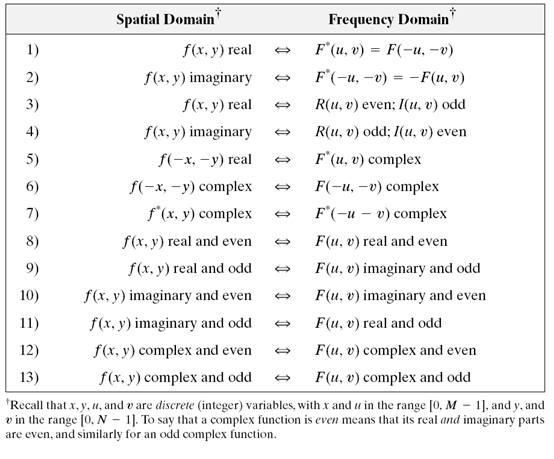
\includegraphics{D:/Documents/GitHub/Commentarii/Digital Image Process Gonzales/1523796663357.png}
\caption{}
\end{figure}

Fourier Spectrum and Phase Angle

Magnitude: Fourier (frequency) spectrum\\
 Power spectrum: \(P(u,v)=|F(u,v)|^2\)

Magnitude, phase angle and power spectrum are arrays of size
\(M\times N\).

\[|F(0,0)|=MN|\bar{f}(x,y)|\text{    where $\bar{f}$ is the average of f}\\
\text{$F(0,0)$ sometimes is called the }\textit{dc component}\]

In general, visual analysis of phase angle images yields little
intuitive information, however, it is a measure of displacement of the
various sinusoids with respect to their origin. The phase is important
in determining shape characteristics.

The 2-D Convolution Theorem

\[f(x,y)*h(x,y)=\sum\limits^{M-1}_{m=0}\sum\limits^{N-1}_{n=0}f(m,n)h(x-m,y-n)\]

gives one period of the convolution, and the following convolution
theorem

\[f(x,y)*h(x,y)\leftrightarrow F(u,v)H(u,v)\\
f(x,y)h(x,y)\leftrightarrow F(u,v)*H(u,v)\]

The first equaiton is the basis for all the filtering techiniques
discussed here.

\(\quad\quad\)If we elect to compute the spatial convolution using the
IDFT of the product of the two transforms, then the periodicity issues
must be taken into account. But \emph{wraparound error} is introduced.

\emph{Zero padding}: by appending to each period enough zeros, the
result would be a correct periodic convolution.

\[f_p(x,y)=\begin{cases}f(x,y) & 0\leq x\leq A-1 \text{ and }0\leq y\leq B-1\\
0 & A\leq x \leq P \text{ or }B\leq y \leq Q \end{cases}\\

h_p(x,y)=\begin{cases}f(x,y) & 0\leq x\leq C-1 \text{ and }0\leq y\leq D-1\\
0 & C\leq x \leq P \text{ or }D\leq y \leq Q \end{cases}\\
\text{with }\ P\geq A+C-1\\Q\geq B+D-1\]

\begin{figure}
\centering
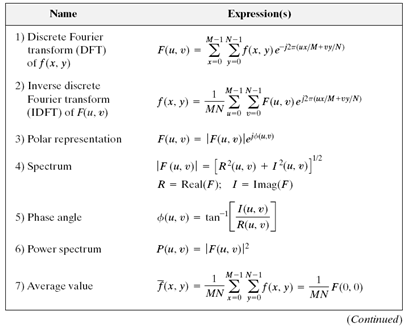
\includegraphics{D:/Documents/GitHub/Commentarii/Digital Image Process Gonzales/1523802270827.png}
\caption{}
\end{figure}

\begin{figure}
\centering
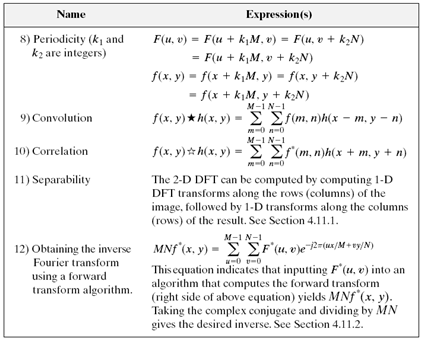
\includegraphics{D:/Documents/GitHub/Commentarii/Digital Image Process Gonzales/1523802284560.png}
\caption{}
\end{figure}

\begin{figure}
\centering
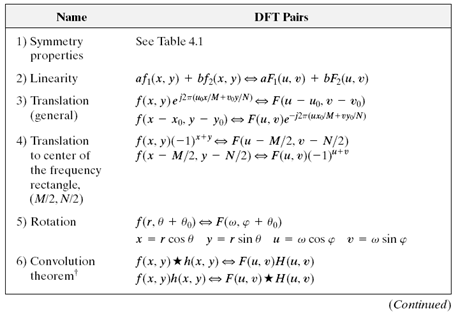
\includegraphics{D:/Documents/GitHub/Commentarii/Digital Image Process Gonzales/1523802307121.png}
\caption{}
\end{figure}

\begin{figure}
\centering
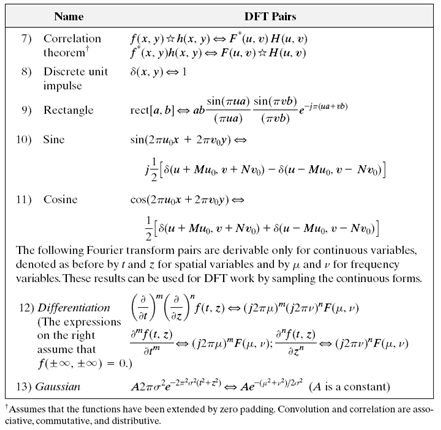
\includegraphics{D:/Documents/GitHub/Commentarii/Digital Image Process Gonzales/1523802320753.png}
\caption{}
\end{figure}

\subsubsection{4.7 The Basics of Filtering in the Frequency
Domain}\label{header-n511}

Intuitive relations between the image domain and the frequency domain.

Fundamentals

\[\text{Given $f(x,y)$ of size $M\times N$}\\
g(x,y)=\mathcal{F^{-1}}[H(u,v)F(u,v)]=\mathcal{F^{-1}}[H(u,v)R(u,v)+jH(u,v)I(u,v)]\]

where \(H(u,v)\) is a filter transfer function.

e.g. \(H(u,v)=0\ for\ u=v=0\ \)otherwise \(1\) reduces the average
intensity Lowpass filter blurs an image while a highpass filter enhance
sharp detail.

The issue on zero padding in the spatial domain\\
 \(\quad\quad\)We cannot work with an infinite number of components, we
cannot use an ideal frequency domain filter and simultaneously use zero
padding to avoid wraparound error. One approach is to zero-pad images
and then create filters in the frequency domain to be of the same size
as the padded images.

\(\quad\quad\)Here we consider only \emph{zero-phase-shift} filters.
Even small changes in the phase angle can have dramtic effects on the
filtered output.

\textbf{Summary}\\

\begin{enumerate}
\def\labelenumi{\arabic{enumi}.}
\item
  Given an input \(f(x,y)\) of size \(M\times N\) and the padding
  parameters \(P\) and \(Q\). Typically \(P=2M\) and \(Q=2N\). Form a
  padded image and multiply \((-1)^{x+y}\) to center its transform,
  compute its DFT.
\item
  Generate a real, symmetric filter function \(H(u,v)\) of size
  \(P\times Q\) with centered at \((P/2, Q/2)\). Form the product
  \(G(i,k)=H(i,k)F(i,k)\).
\item
  Obtain the porcessed image \\

  \[g_p (x,y)=\{real[\mathcal{F}^{-1}[G(u,v)]]\}(-1)^{x+y}\]

  where the real part is selected to ignore parasitic complex components
  resulting from computational inaccuracies.
\item
  Extract the original region.
\end{enumerate}

Correspondence Between Filtering in the Spatial and Frequency Domains

\[h(x,y)\leftrightarrow H(u,v)\]

\(h(x,y)\) is sometiems referred as the \emph{impulse response}. Since
all quantities in a discrete implementation are finite, such filters are
called \emph{finite impulse response (FIR)} filters.

\$\textbackslash{}quad\textbackslash{}quad\$Spatial convolution in terms
of the convolution theorem and the DFT implies convolving periodic
functions, involving functions of the same size.

\$\textbackslash{}quad\textbackslash{}quad\$In practice, we prefer to
implement convolution filtering with small filter masks because of speed
and ease of implementation. But we can specify a filter in the frequency
domain, compute its IDFT, and use the resulting full-size spatial filter
as a guide for constructing smaller spatial filter masks. The other way
around, a small spatial filter is given and its full-size frequency
domain representation is obtained to analyze the behavior of the small
spatial filters in the frequency domain.

\$\textbackslash{}quad\textbackslash{}quad\$The forward way: design a
spatial filter by analyze a frequency filter\\
 An example of Gaussian filter, a lowpass filter and a highpass filter
obtained through difference of two Gaussian filter.

\$\textbackslash{}quad\textbackslash{}quad\$The backward way: start with
a spatial mask and generate its corresponding filter in the frequency
domain.

\subsubsection{4.8 Image Smoothing Using Frequency Domain
Filters}\label{header-n556}

\(\quad\quad\)Smoothing is achieved by high-frequency attenuation
(lowpass filtering).

Ideal Lowpass Filters

\(\quad\quad\)A cylinder centered at \((M/2,P/2)\).

\emph{Cut-off frequency}: determined by the power encircled by the
cylinder w.r.t. the whole power spectrum.

Butterworth Lowpass Filter

\[H(u,v)=\dfrac{1}{1+\big(D(u,v)/D_0\big)^{2n}}\]

where \(D_0\) is the distance at which cutoff frequency (\(H(D_0)=0.5\))
is from the origin. The higher the order is, the more significant the
"ringing" (waving) in the spatial domain. BLPFs of order 2 are a good
compromise between effective lowpass filterign and acceptable ringing.

Gaussian Lowpass Filters

\[H(u,v)=e^{-D^2(u,v)/2D_0^2}\]

where \(D(u,v)\) is a distance function. The inverse Fourier transform
of the GLPFs is Gaussian too, which has no "ringing".

\(\quad\quad\)Lowpass filtering in Character Recognition preprocessing.

\subsubsection{4.9 Image Sharpening Using Frequency Domain
Filters}\label{header-n574}

\(\quad\quad\)A highpass filter is obtained from a given lowpass filter
using the equation

\[H_{HP}(u,v)=1-H_{LP}(u,v)\]

Ideal Highpass Filters

Butterworth Highpass Filters

\[H(u,v)=\dfrac{1}{1+\big(D_0/D(u,v)\big)^{2n}}\]

Gaussian Highpass Filters

\[H(u,v)=1-e^{-D^2(u,v)/2D_0^2}\]

The Laplacian in the Frequency Domain

\[H(u,v)=-4\pi^2(u^2+v^2)\\
H(u,v)=-4\pi^2D^2(u,v)\]

Unsharp Masking, Highboost Filtering, and High-Frequency-Emphasis
Filtering

\[g_{mask}(x,y)=f(x,y)-f_{LP}(x,y)\\
f_{LP}(x,y)=\mathcal{F}^{-1}\Big(H_{LP}(u,v)F(u,v)\Big)\]

\textbf{High-frequency-emphasis filter}:
\(g(x,y)=\mathcal{F}^{-1}\Bigg(\Big[k_1+k_2*H_{HP}(u,v)\Big]F(u,v)\Bigg)\)

where \(k_1\geq 0 \) gives controls of the offset from the origin and
\(k_2\) controls the contribution of high frequencies.

Homomorphic Filtering

\begin{figure}
\centering
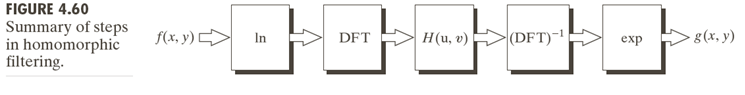
\includegraphics{D:/Documents/GitHub/Commentarii/Digital Image Process Gonzales/1524389122153.png}
\caption{}
\end{figure}

The \emph{illumination} component is characterized by slow spatial
variations while the \emph{reflectance} component tends to vary
abruptly, particularly at the junctions of dissimilar objects.

\subsubsection{4.10 Selective Filtering}\label{header-n596}

Bandreject and Bandpass Filters (A cirle, a sphere)

\[H_{BP}(u,v)=1-H_{BR}(u,v)\]

\begin{figure}
\centering
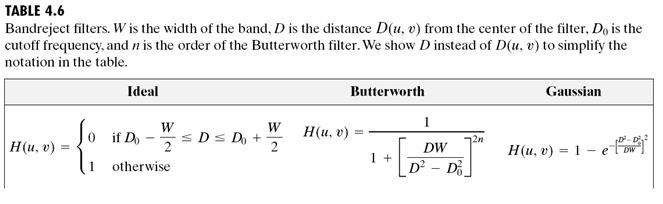
\includegraphics{D:/Documents/GitHub/Commentarii/Digital Image Process Gonzales/1524389588133.png}
\caption{}
\end{figure}

Notch Filters (small regions in the frequency domain)

\[H_{NR}(u,v)=\prod\limits^{Q}_{k=1}H_k(u,v)H_{-k}(u,v)\]

where \(H_k(u,v)\) and \(H_{-k}(u,v)\) are highpass filters whose
centers are at \((u_k,v_k)\) and \((-u_k, -v_k)\) respectively.

\[H_{NP}(u,v)=1-H_{NR}(u,v)\]

\section{Chap.5 Image Restoration and Reconstruction}\label{header-n606}

\(\quad\quad\)The principal goal of restoration techniques is to improve
an image in some predefined sense. Image enhancement is largely a
subjective process, while restoration attempts to recover an image that
has been degraded by using a priori knowledge of the degradation
phenomenon, that is, oriented toward modeling the degradation and
applying the inverse process in order to recover the original image.

\textbf{A Model of the Image Degradation/Restoration Process}

\[g(x,y)=h(x,y)*f(x,y)+\eta(x,y)\\
G(u,v)=H(u,v)F(u,v)+N(u,v)\]

\subsection{5.2 Noise Model}\label{header-n612}

Arising during image acquisition and or transmission.

Spatial and Frequency Properties of Noise

\emph{White noise}: constant Fourier spectrum

\$\textbackslash{}quad\textbackslash{}quad\$In the discussion below we
consider the noise uncorrelated w.r.t the image itself, independent of
its spatial coordinates, though this is not always the case in reality.

Some Important Noise Probability Density Functions

\textbf{Gaussian Noise}

\[p(z)=\dfrac{1}{\sqrt{2 \pi} \sigma}e^{-(z-\bar{z})^2/2\sigma^2}\]

where \(z\) represents intensity. \(70\%\) in
\((\bar{z}-\sigma,\bar{z}+\sigma)\) and \(95\%\) in
\((\bar{z}-2\sigma,\bar{z}+2\sigma)\)

\textbf{Rayleigh noise}

\[p(z)=\begin{cases}\dfrac{2}{b}(z-a)e^{-(z-a)^2/b}&\text{for }\ z\geq a\\0 & \text{for} \ \ z<a\end{cases}\]

mean and variance given by

\[\bar{z}=a+\sqrt{\pi b/4}\\
\sigma^2=\dfrac{b(4-\pi)}{4}\]

Skewed to the right, quite useful for approximating skewed histograms.

\textbf{Erlang noise}

\[p(z)=\begin{cases}\dfrac{a^b z^{b-1}}{(b-1)!}e^{-az}&for\ z\geq 0\\
0&for\ z<0\end{cases}\]

Mean \(\bar{z}=\dfrac{b}{a}\) and variance \(\sigma^2=\dfrac{b}{a^2}\)

Referred as the \emph{gamma density} only when the denominator is the
\emph{gamma function}
\href{https://en.wikipedia.org/wiki/Gamma_function}{Gamma Funciton}\\

\href{https://en.wikipedia.org/wiki/Factorial\#Extension_of_factorial_to_non-integer_values_of_argument}{Gamma
Function and Factorial}\\
 \href{https://en.wikipedia.org/wiki/Gamma_distribution}{Gamma
distribution}

\textbf{Exponential noise}

\[p(z)=\begin{cases}ae^{-az} & for\ z\geq 0\\0 & for\ z<0 \end{cases}\]

where \(a>0\)

mean \(\bar{z}=\dfrac{1}{a}\) and variance \(\sigma^2=\dfrac{1}{a^2}\)

A special case of the Erlang with \(b=1\)

\textbf{Uniform noise}

\textbf{Impulse (salt-and-pepper) noise}

\emph{bipolar impulse}

\[p(z)=\begin{cases}P_a & for\ z=a\\P_b & for\ z=b\\ 0 & otherwise\end{cases}\]

if either of \(P_a, P_b\) is zero, the impulse noise is called
\emph{unipolar}

If neigther is zero and especially approximately equal,
\emph{salt-and-pepper} , \emph{data-drop-out} or \emph{spike}.

\(a\) and \(b\) are usually assumed to be saturated values, either black
or white.

\begin{figure}
\centering
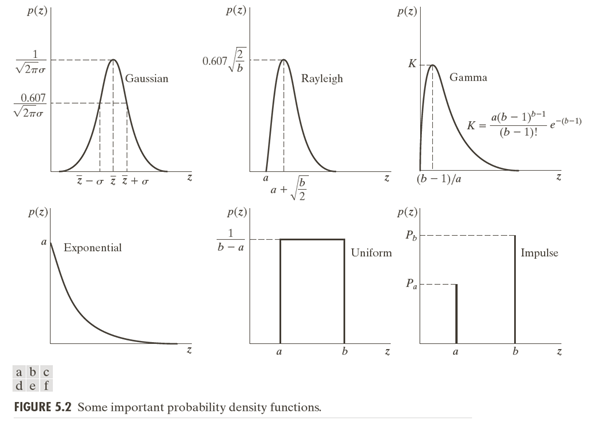
\includegraphics{D:/Documents/GitHub/Commentarii/Digital Image Process Gonzales/1524044319176.png}
\caption{}
\end{figure}

Periodic Noise

Arising typically from electrical or electromechanical interference
during image acquisition and can be reduced significantly via frequency
domain filtering.

Estimation of Noise Parameters

If the imaging system is available, one simple way to study the
characteristics of system noise is to capture a set of images of "flat"
environments. It is possible to estimate the parameters of the PDF from
small patches of reasonably constant background intensity.

\subsection{5.3 Restoration in the Presence of Noise Only - Spatial
Filtering}\label{header-n673}

\(\quad\quad\)It is usually possible to estimate noise from the
spectrum.

\(\quad\quad\)Spatial filtering is the method of choice in situations
when only addtive random noise is present.

Mean Filters

\textbf{Arithmetic mean filter}

\[\hat{f}(x,y)=\dfrac{1}{mn}\sum\limits_{(s,t)\in S_{xy}}g(s,t)\]

\textbf{Geometric mean filter}

\[\hat{f}(x,y)=\Bigg(\prod\limits_{(s,t)\in S_{xy}}g(s,t)\Bigg)^{\frac{1}{mn}}\]

It tends to lose less image detail compared to the arithmetic mean
filter.

\textbf{Harmonic mean filter}

\[\hat{f}(x,y)=\dfrac{mn}{\sum\limits_{(s,t)\in S_{xy}}\frac{1}{g(s,t)}}\]

Works well for salt noise and other types like Gaussian noise, but fails
for pepper noise.

\textbf{Contraharmonic mean filter}

\[\hat{f}(x,y)=\dfrac{\sum\limits_{(s,t)\in S_{xy}}g(s,t)^{Q+1}}{\sum\limits_{(s,t)\in S_{xy}}g(s,t)^{Q}}\]

where \(Q\) is called the order of the filter. Well suited for reducing
or virtually eliminating the effects of salt-and-pepper noise.

For positive Q, it eleminates pepper noise.\\
 For negative Q, salt noise.\\
 It cannot do both simultaneously.

It reduces to arithmetic filter if \(Q=0\) and to the harmonic mean
filter if \(Q=-1\)

\(\quad\quad\)In general, the arithmetic and geometric mean filters
(particularly the latter) are well suited for random noise like Gaussian
or uniform. The contraharmonic is well suited for impulse noise.

Order-Statistic Filters

\textbf{Median Filter}

\[f(x,y)=\underset{(s,t)\in S_{xy}}{median}\{g(s,t)\}\]

Best-known order-statistic filter, particularly effective in the
presence of both bopolar and unipolar impulse noise. It can be used
repeatedly (Note that it could blur the image).

\textbf{Max and min filters}

\emph{Max}: useful for finding the brightest points, reducing pepper
noise.\\
 \emph{Min}: darkest points, reducing salt noise.

\textbf{Midpoint filter}

\[\hat{f}(x,y)=\dfrac{1}{2}\Bigg(\underset{(s,t)\in S_{xy}}{max}\{g(s,t)\}+\underset{(s,t)\in S_{xy}}{min}\{g(s,t)\}\Bigg)\]

Works best for randomly distributed noise like Gaussian or uniform.

\textbf{Alpha-trimmed mean filter}

\[\hat{f}(x,y)=\dfrac{1}{mn-d}\sum\limits_{(s,t)\in S_{xy}}g_r(s,t)\]

where \(g_r(s,t)\) represents the remaining pixels after deleting the
lowest \(d/2\) and the highest \(d/2\) pixels, and \(d\) ranges from
\(0\) to \(mn-1\). When \(d=mn-1\), the filter becomes a median filter.
Useful in situations involving multiple types of noise, such as a
combination of salt-and-pepper and Gaussian noise.

Adaptive Filters

\textbf{Adaptive, local noise reduction filter}

Mean and variance are reasonable parameters on which to base an adaptive
fitler because they are quantities closely related to the appearance of
an image.

Four parameters to be considered\\

\begin{enumerate}
\def\labelenumi{\arabic{enumi}.}
\item
  \(g(x,y)\) the value of the noisy image at \((x,y)\)
\item
  \(\sigma^2_{\eta}\) the variance of the noise
\item
  \(m_L\) the local mean of the neighborhood
\item
  \(\sigma_L^2\) the local variance
\end{enumerate}

Behavior of the filter\\

\begin{enumerate}
\def\labelenumi{\arabic{enumi}.}
\item
  If \(\sigma_\eta^2=0\), zero-noise case in which \(g(x,y)=f(x,y)\) 
\item
  If \(\sigma_L^2 \gg \sigma_\eta^2\), this is typically associated with
  edges that should be preserved.
\item
  If the two variances are equal, local area has the same properties as
  the overall image, and local noise is to be reduced simply by
  averaging. 
\end{enumerate}

Result:

\[\hat{f}(x,y)=g(x,y)-\dfrac{\sigma_\eta^2}{\sigma^2_L}\Big(g(x,y)-m_L\Big)\]

Set the ratio to \(1\) if the condition \(\sigma_\eta^2>\sigma_L^2\)

\textbf{Adaptive median filter}

\(\quad\quad\)The adaptive median filtering can handle impulse noise
with large spatial densities and preserve detail while smoothing
nonimpulse noise.

\[z:\text{intensity value in the neighborhood $S_{xy}$}, \ z_{min},\ z_{max},\ z_{med},\ z_{xy}, \\S_{max}\text{: maximum allowed size of $S_{xy}$}\]

\emph{Algorithm}: \\
 Stage A: \(A1 = z_{med}-z_{min}\)\\
 \(A2 = z_{med}-z_{max}\) \\
 If \(A1>0\) AND \(A2<0\), go to stage B\\
 Else increase \(S_{xy}\)\\
 If \(S_{xy}\leq S_{max}\) repeat stage A\\
 Else output \(z_{med}\)\\

 Stage B: \(B1=z_{xy}-z_{min}\)\\
 \(B2=z_{xy}-z_{max}\)\\
 If \(B1>0\) AND \(B2<0\), output \(z_{xy}\)\\
 Else output \(z_{med}\)

It removes salt-and-pepper noise, provides smoothing of other noise that
may not be impulsive and to reduce distortion.

\(z_{min}\) and \(z_{max}\) are considered statistically the impulse
noise value. Stage A Line 3 and Stage B check if the respective values
are impulses. The smaller the \(P_a\) or \(P_b\), the larger \(S_{max}\)
is allowed to be.

\subsection{5.4 Periodic Noise Reduction by Frequency Domain
Filtering}\label{header-n785}

\(\quad\quad\)Periodic noise appears as concentrated bursts of energy in
the FT, at locations corresponding to the frequencies of the periodic
interference. The approach is to use a selective filter to isolate the
noise.

Bandreject Filters

Bandpass Filters

Useful because it simplifies analysis of the noise, reasonably
independent of image content.

Notch filters

Optimum Notch Filtering

\(\quad\quad\)The interference components generally are not
single-frequency bursts. Instead they tend to have broad skirts that
carry information about the interference pattern.

\(\quad\quad\)The first step is to extract the principal frequency
components of the interference pattern by \(N(u,v)=H_{NP}(u,v)G(u,v)\)
and obtain its spatial expression
\(\eta(x,y)=\mathcal{F}^{-1}\{H_{NP}(u,v)G(u,v)\}\).

\(\quad\quad\)The estimate of \(f(x,y)\):
\(\hat{f}(x,y)=g(x,y)-w(x,y)\eta(x,y)\), the function \(\eta(x,y)\)
called \emph{weighting} or \emph{modulation} function. The objective of
the procedure is to select this funciton so that the result is optimized
in some meaningful way.

\(\quad\quad\)If we choose to mimimize the variance of the estimate
\(\hat{f}(x,y)\) over a specified neighborhood, we have the following
result.

\[w(x,y)=\dfrac{\overline{g(x,y)\eta(x,y)}-\bar{g}(x,y)\bar{\eta}(x,y)}{\bar{\eta^2}(x,y)-\bar{\eta}^2(x,y)}\]

\(w(x,y)\) is assumed to be constant in a neighborhood.

\subsection{5.5 Linear, Position-Invariant
Degradations}\label{header-n805}

\[g(x,y)=H[f(x,y)]+\eta(x,y)\\
\quad\quad\quad\text{Linearity:  } H[af_1(x,y)+bf_2(x,y)]=aH[f_1(x,y)]+bH[f_2(x,y)]\\
\text{Position invariant: } H[f(x-\alpha, y-\beta)]=g(x-\alpha, y-\beta)\]

\[\qquad \qquad \quad g(x,y)=\int^{\infin}_{-\infin}\int^{\infin}_{-\infin}f(\alpha,\beta)h(x,\alpha,y,\beta)d\alpha d\beta\ +\ \eta(x,y)\\
 = h(x,y)*f(x,y) + \eta(x,y)\\
 G(u,v)=H(u,v)F(u,v)+N(u,v)\]

where \(h(x,\alpha,y,\beta)\) is the \emph{impulse response} of \(H\).
Assume \(H\) is position-invariant, it becomes \(h(x-\alpha, y-\beta)\).

\(\quad\quad\)The term \emph{image deconvolution} is used to signify
\emph{linear image restoration}, and the filters in the process are
called \emph{deconvolution filters}.

\subsection{5.6 Estimating the Degradation Function}\label{header-n812}

\(\quad\quad\)The process of restoring an image by using a degradation
function that has been estimated in some way sometimes is called
\emph{blind convolution}, since the true degradation function is seldom
known completely.

Estimation by Image Observation

\(\quad\quad\)A laborious process used only in very specific
circumstances such as, for example restoring an old photograph of
historical value.

Estimation by Experimentation

\(\quad\quad\)If equipment similar to the equipment used to acquire the
degraded image is available, it is possible in principle to obtain an
accurate estimate of the degradation. The idea is to obtain the impulse
response of the degradation by imaging an impulse (small dot of light)
using the same system settings.

Estimation by Modeling

\(\quad\quad\)Take into account environmental conditions that cause
degradations.

E.g. The Gaussian lowpass filter is used sometimes to model mild,
uniform blurring.

Another major approach in modeling is to derive a mathematical model
starting from basic principles.

E.g. An example of blurring due to continuous exposure.

\subsection{5.7 Inverse Filtering}\label{header-n830}

\[\hat{F}(u,v)=F(u,v)+\dfrac{N(u,v)}{H(u,v)}\]

Even if we know the degradation function we cannot recover the
undegraded image exactly becuase \(N(u,v)\) is not known. If the
degradation function has zero or very small values, then the ratio
\(N(u,v)/H(u,v)\) could easily dominate the estimate \(\hat{F}(u,v)\).
One apporach to avoid the zero or small-value problem is to limit the
filter frequencies to values near the origin, assuming \(H(u,v)\) has
the hightest value at the origin.

\subsection{5.8 Minimum Mean Square Error (Wiener)
Filtering}\label{header-n834}

\(\quad\quad\) Wiener Filtering takes into account the noise. The methdo
is founded on considering images and noise as random variables and the
objective is to find an estimate that minimizes
\(e^2=E\{(f-\hat{f})^2\}\), and it yields the following result:

\[\hat{F}(u,v)=\Bigg[\dfrac{1}{H(u,v)}\dfrac{|H(u,v)|^2}{|H(u,v)|^2+S_\eta(u,v)/S_f(u,v)}\Bigg]G(u,v)\]

where \(S_\eta(u,v)=|N(u,v)|^2=\) power spectrum of the noise\\
 \(S_f(u,v)=|F(u,v)|^2=\) power spectrum of the undegraded image

This "two S's" term can be measured by \emph{signal-to-noise ratio}
\(SNR=\dfrac{\sum\limits^{M-1}_{u=0}\sum\limits^{N-1}_{v=0}|F(u,v)|^2}{\sum\limits^{M-1}_{u=0}\sum\limits^{N-1}_{v=0}|N(u,v)|^2}\)

The noise term may be replaced with
\(MSE=\dfrac{1}{MN}\sum\limits^{M-1}_{x=0}\sum\limits^{N-1}_{y=0}\big[f(x,y)-\hat{f}(x,y)\big]^2\)

The power spectrum of the undegraded image seldom is known. An approach
frequently used is to approximate by a constant \(K\).

\[\hat{F}(u,v)=\Bigg[\dfrac{1}{H(u,v)}\dfrac{|H(u,v)|^2}{|H(u,v)|^2+K}\Bigg]G(u,v)\]

\subsection{5.9 Constrained Least Squares Filtering}\label{header-n848}

\(\quad\quad\)A constant estimate of the ratio of the power spectra for
Wiener filters is not always a suitable solution. The method here
requires knowledge of only the \emph{mean} and \emph{variance} of the
noise, which are usually calculated easily from the degraded image.
Wiener filter is optimal in an average sense, but not for each image.

\[g=Hf+\eta\]

Optimization problem

\[C=\sum\limits^{M-1}_{x=0}\sum\limits^{N-1}_{y=0}\big[\triangledown^2f(x,y)\big]^2\]

subject to the constraint

\[||g-H\hat{f}||^2=||\eta||^2\]

solution given by

\[\hat{F}(u,v)=\Bigg[\dfrac{H^*(u,v)}{|H(u,v)|^2+\gamma|P(u,v)|^2}\Bigg]G(u,v)\]

where \(\gamma\) is a parameter that must be adjusted to satisfy
Eq.(86), and \(P(u,v)\) is the FT of the Laplacian operator.

\(\quad\quad\)To determine the best \(\gamma\), define a residual vector

\[\vec{r}=\vec{g}-H\vec{\hat{f}}=\vec{\eta}\]

The objective function \(\phi(r)=||r||^2\) is a monotonically increasing
function of \(\gamma\). We want to adjust \(\gamma\) so that
\(||r||^2=||\eta||^2\pm a\), where \(a\) is an accuracy factor. This
optimization can be solved iteratively. Given an initial \(\gamma_{0}\),
using Eq.(87) and (89) to compute the current \(r\).

\[||r||^2=\sum\limits^{M-1}_{x=0}\sum\limits^{N-1}_{y=0}r^2(x,y)\]

where \(r(x,y)=\mathcal{F}^{-1}[R(u,v)]\) and
\(R(u,v)=G(u,v)-H(u,v)\hat{F}(u,v)\).

Since

\[\sigma^2_\eta=\dfrac{1}{MN}\sum\limits^{M-1}_{x=0}\sum\limits^{N-1}_{y=0}\big[\eta(x,y)-m_\eta \big]^2\]

Expand Eq.(88) and we have

\[||\eta||^2=MN[\sigma_\eta^2+m^2_\eta]\]

\subsection{5.10 Geometric Mean Filter}\label{header-n877}

\textbackslash{}indA generalization of Wiener filter, called
\emph{geometric mean filter}:

\[\hat{F}(u,v)=\Bigg[\dfrac{H^*(u,v)}{|H*(u,v)|^2}\Bigg]^\alpha\Bigg[\dfrac{H^*(u,v)}{|H(u,v)|^2+\beta\big[\frac{S_\eta(u,v)}{S_f(u,v)}]}\Bigg]^{1-\alpha}G(u,v)\]

\(\alpha=1\): inverse filter\\
 \(\alpha =0\): parametric Wiener filter\\
 \(\alpha=1/2\) and \(\beta=1\): spectrum equailzaition filter.

\end{document}
